\documentclass[tikz]{standalone}

\colorlet{FilledSurface}{blue!20}
\colorlet{FilledSurfaceGroupOne}{blue!20}
\colorlet{FilledSurfaceGroupTwo}{red!20}
\colorlet{FilledSurfaceGroupThree}{green!20}
\colorlet{FilledSurfaceGroupFour}{magenta!20}
\colorlet{FormulaBackground}{green!10}
\colorlet{FormulaFrame}{green}


\usetikzlibrary{calc, decorations.markings, arrows.meta}

\tikzset{
    mark rect/.style={
        decoration={markings, mark=at position 0.5 with {
            \draw[draw=black, fill=white] (-6pt,-2pt) rectangle (6pt,2pt);
        }}, postaction={decorate}
    },
    mark two circles/.style={
        decoration={markings, mark=at position 0.5 with {
                \draw[fill=white] (-2pt,0) circle (2pt);
                \draw[fill=white] (2pt,0) circle (2pt);
        }}, postaction={decorate}
    }
}

\usepackage{tikz-dimline}

\begin{document}
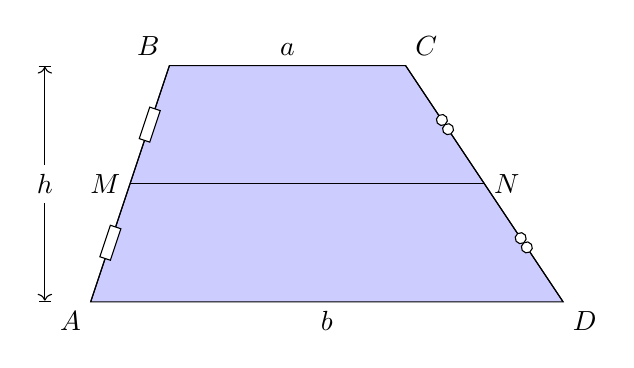
\begin{tikzpicture}

\coordinate (A) at (0, 0);
\coordinate (B) at (1, 3);
\coordinate (C) at (4, 3);
\coordinate (D) at (6, 0);
\draw[fill=FilledSurfaceGroupOne]
    (A) node[below left]{$A$}
    -- (B) node[above left]{$B$}
    -- node [above]{$a$} (C) node[above right]{$C$}
    -- (D) node[below right]{$D$}
    -- node [below]{$b$}cycle;


\coordinate (M) at ($(A)!0.5!(B)$);
\coordinate (N) at ($(C)!0.5!(D)$);

\draw (M) node [left]{$M$} -- (N) node [right]{$N$};

\draw[mark rect] (A) -- (M);
\draw[mark rect] (B) -- (M);
\draw[mark two circles] (C) -- (N);
\draw[mark two circles] (D) -- (N);

% The notation "|-" does the following:
% Find the point that has the x-coordinate of B and the y-coordinate of A.
% Find the projection of point B onto a horizontal line passing through point A.
\coordinate (Bproj) at (B |- A);

\draw[color = black,|<->|] ($(B)!45pt!-90:(Bproj)$) to node [fill=white, midway] {$h$} ($(Bproj)!45pt!90:(B)$);

\end{tikzpicture}
\end{document}

